\باب{مویج اور گھمکیا}\شناخت{باب_مویج}
اب تک ہم صرف \اصطلاح{عرضی برقی و مقناطیسی}\فرہنگ{عرضی!برقی و مقناطیسی}\حاشیہب{transverse electromagnetic, TEM}\فرہنگ{transverse electromagnetic}\فرہنگ{TEM}  \تحریر{TEM} امواج کی بات کرتے آ رہے ہیں جن میں برقی اور مقناطیسی دونوں میدان سمت حرکت کے عمودی ہوتے ہیں۔اس باب میں ترسیلی تار پر بحث کو آگے بڑھاتے ہوئے ایسے امواج پر غور کیا جائے گا جن میں برقی یا مقناطیسی میدان سمت حرکت کی جانب بھی جزو رکھتے ہوں۔وہ ترسیلی تار جو صرف اس طرح کے امواج کو گزار سیکھیں \اصطلاح{میوج}\فرہنگ{مویج}\حاشیہب{waveguide}\فرہنگ{waveguide} کہلاتے ہیں۔

دو لامحدود جسامت کے مستوی سطحوں کے مویج سے بات شروع کرتے ہوئے کھوکھلے مستطیلی اور نلکی مویج تک بات بڑھائی جائے گی۔ان مویج میں میدان کے اشکال، ان کے منقطع طول موج اور تقلیلی مستقل  حاصل کئے جائیں گے۔اس کے بعد ایک تار پر بیرونی موج اور دیگر اقسام کے مویج پر غور کیا جائے گا۔آخر میں موصل کے بند ڈبوں میں قید امواج پر غور کیا جائے گا جنہیں گھمکیا کہتے ہیں۔

\حصہ{برقی دور، ترسیلی تار اور مویج کا موازنہ}
کم تعدد پر برقی دباو، برقی رو، مزاحمت وغیرہ عملی متغیر ہیں جنہیں استعمال کرتے ہوئے برقی ادوار حل کئے جاتے ہیں۔ان تعدد پر تمام مزاحمت یا رکاوٹ کو نقطہ نما تصور کیا جاتا ہے۔یوں تار کے ایک سرے پر منبع برقی دباو لاگو کرتے ہوئے تار کے دوسرے سرے پر مزاحمت میں برقی رو حاصل کی جا سکتی ہے۔

قدر زیادہ تعدد پر انہیں حقائق کو ترسیلی تار پر لاگو کیا جا سکتا ہے۔ایسا کرتے وقت ترسیلی تار کی مزاحمت یا امالہ تار کی لمبائی پر تقسیم شدہ  تصور کرنا لازم ہے۔ساتھ ہی ساتھ ترسیلی تار پر برقی دباو کی رفتار پر بھی نظر رکھنی ہوتی ہے۔

اب موصل کھوکھلے نلکی یا مستطیلی نالی پر مبنی نظام کی بات کرتے ہیں۔کیا ایسی نالی برقی و مقناطیسی طاقت منتقل کرنے کی صلاحیت رکھتی ہے؟ اگر ہماری معلومات برقی ادوار یا ترسیلی تار تک محدود ہوتی تب اس سوال کا جواب یہ ہے کہ ایسا ممکن نہیں ہے کیونکہ برقی طاقت کے منتقلی کے لئے دو تار ضروری ہیں۔البتہ اگر ہم شعاعوں کا علم رکھتے تب جواب ہوتا کہ ایسا ممکن ہے چونکہ شعاعیں سیدھی کھوکھلے نلکی سے گزر سکتی ہیں اور شعاعیں بلند تعدد \عددیء{(\SI{e16}{\hertz})} کی برقی و مقناطیسی امواج ہی ہیں۔

اصل جواب ہے کہ ایسا امواج کے تعدد پر منحصر ہے۔کم تعدد کے امواج نالی سے نہیں گزر سکتے جبکہ بلند تعدد کے امواج اس سے گزر سکتے ہیں۔تعدد کے ان دو خطوں کے درمیان ایسی تعدد ہو گی جس سے کم تعدد نالی سے نہیں گزرے گی اور جس سے زیادہ تعدد نالی سے گزرے گی۔اس تعدد کو \اصطلاح{پست انقطاعی تعدد}\فرہنگ{تعدد!پست انقطاعی}\فرہنگ{انقطاعی!پست تعدد}\حاشیہب{low cutoff frequency}\فرہنگ{frequency!low cutoff} کہا جاتا ہے۔ 

کھوکھلے نالی سے برقی و مقناطیسی طاقت کی منتقلی برقی ادوار حل کرنے کے علم سے ناقابل سمجھ مسئلہ ہے۔کھوکھلے نالی میں طاقت کی منتقلی، نالی کے کھوکھلے حصے میں برقی اور مقناطیسی میدان پر غور سے سمجھا جا سکتا ہے جنہیں استعمال کرتے ہوئے  پوئنٹنگ سمتیہ سے موج کی طاقت حاصل ہوتی ہے۔دراصل برقی و مقناطیسی طاقت نالی کے کھوکھلے حصے میں برقی اور مقناطیسی امواج سے منتقل ہوتا ہے نا کہ نالی کے موصل حصے میں۔برقی دباو اور برقی رو اس منتقلی کے محض اضافی اثرات ہیں۔ 

\حصہ{دو لامحدود وسعت کے مستوی چادروں کے مویج میں عرضی برقی موج}
شکل \حوالہ{شکل_مویج_لامحدود_متوازی_چادر} میں دو لامحدود وسعت کے متوازی چادروں پر مبنی ترسیلی تار دکھائی گئی ہے جو \عددیء{y} سمتی عرضی برقی و مقناطیسی موج گزار سکتی
 ہے۔ اس تار کی خاص خاصیت یہ ہے کہ ایک مخصوص تعدد کے اوپر یہ دیگر \اصطلاح{بلند درجی انداز}\فرہنگ{انداز!بلند درجی}\حاشیہب{higher order mode}\فرہنگ{mode!higher order} کے امواج بھی گزار سکتی ہے۔یوں ترسیلی تار سے شروع کرتے ہوئے مویج تک بحث کو پہنچانے  کے لئے یہ بہترین مثال ہے۔

\begin{figure}
\centering
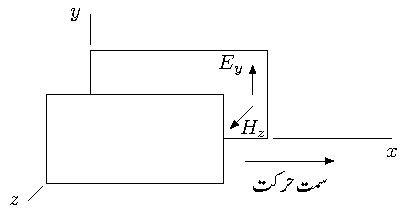
\includegraphics{figWaveguidesInfiniteParallelPlates}
\caption{دو لامحدود وسعت کے متوازی موصل چادروں کا نظام۔}
\label{شکل_مویج_لامحدود_متوازی_چادر}
\end{figure}

ایسی بلند درجی انداز کی بات کرتے ہیں جس میں برقی میدان ہر نقطے پر \عددیء{y} سمتی ہے جبکہ سمت حرکت \عددیء{\ax} ہے۔چونکہ برقی میدان سمت حرکت کے عمودی ہے لہٰذا اس انداز کو \اصطلاح{عرضی برقی انداز}\فرہنگ{عرضی!برقی انداز}\فرہنگ{انداز!عرضی برقی}\حاشیہب{transverse electric mode, TE mode}\فرہنگ{transverse electric mode}\فرہنگ{mode, transverse electric, TE} \تحریر{(TE)} کہا جائے گا۔اگرچہ اس موج میں برقی میدان عرضی ہے، مقناطیسی میدان عرضی اور طولی اجزاء پر مشتمل ہے۔کامل موصل چادروں کی صورت میں چادروں پر برقی میدان صفر ہو گا البتہ چادر سے دور  اس کی کچھ بھی قیمت ممکن ہے۔ایسی عرضی برقی انداز موج کے خصوصیات باآسانی یوں حاصل کئے جا سکتے ہیں کہ اسے دو عرضی برقی و مقناطیسی انداز \تحریر{TEM} امواج کا مجموعہ تصور کیا جائے جو موصل چادروں کے درمیان بار بار انعکاس کرتی ہوں۔

آئیں پہلے شکل \حوالہ{شکل_مویج_دو_عرضی_امواج_خالی_خلاء} پر غور کریں جہاں خالی خلاء میں ایک ہی تعدد کے دو سطحی \تحریر{TEM} امواج کے ملاپ کی صورت حال دکھائی گئی ہے۔اس شکل میں امواج خطی قطبی تصور کئے گئے ہیں جن کا برقی میدان صفحہ کے عمودی فرض کیا گیا ہے۔موج الف کی شعاع اوپر بائیں ہاتھ سے نیچے دائیں ہاتھ کی طرف جبکہ موج ب کی شعاع نیچے بائیں ہاتھ سے اوپر دائیں ہاتھ کی جانب گامزن ہے۔یوں ان کا آپس میں ملاپ کسی زاویے پر ہوتا ہے۔شکل میں گہری سیاہی کی ٹھوس لکیر سے موج کی چوٹی جبکہ ہلکی سیاہی کے ٹھوس لکیر سے اس کا نشیب دکھایا گیا ہے۔یوں سطحی موج الف کی چوٹیاں اور نشیب، شعاع الف کے عمودی دکھائے گئے ہیں۔گہری سیاہی کے ٹھوس لکیر کو برقی میدان کی چوٹی تصور کیا جائے۔یوں اس لکیر پر برقی میدان زیادہ سے زیادہ قیمت رکھتا ہے اور اس کی سمت صفحہ سے عمودی باہر جانب کو ہے۔اسی طرح ہلکی ٹھوس لکیر میدان کی نشیب کو ظاہر کرتی ہے لہٰذا یہاں میدان کی قیمت زیادہ سے زیادہ ہو گی البتہ اس کی سمت صفحہ کے عمودی اندر جانب کو ہو گی۔چوٹی اور نشیب کے درمیان فاصلہ \عددیء{\tfrac{\lambda_0}{2}} کے برابر ہے۔ 
%
\begin{figure}
\centering
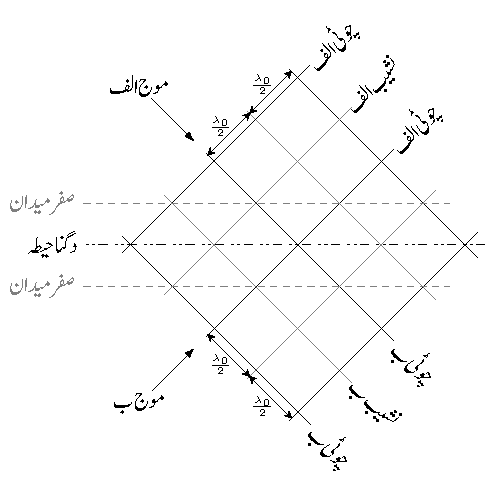
\includegraphics{figWaveguidesTwoIntersectingTEMwaves}
\caption{دو عرضی برقی و مقناطیسی امواج خلاء میں مختلف سمتوں میں حرکت کر رہی ہیں۔}
\label{شکل_مویج_دو_عرضی_امواج_خالی_خلاء}
\end{figure}

جس نقطے پر ایک موج کی چوٹی اور دوسری موج کا نشیب ملتے ہیں اس نقطے پر کل میدان صفر کے برابر ہو گا۔یوں جہاں گہری سیاہی اور ہلکی سیاہی کے لکیر ملتے ہیں وہاں میدان صفر ہو گا۔شکل میں ہلکی سیاہی میں ایسی دو نقطہ دار لکیریں کھینچی گئی ہیں جن پر میدان صفر کے برابر ہے۔آپ غور کر کے تسلی کر لیں کہ ان لکیروں کے ہر نقطے پر برقی میدان صفر ہی ہے۔مزید آپ ذہن میں دونوں امواج کو حرکت دیتے ہوئے تسلی کر لیں کہ امواج کے حرکت کے باوجود ان دو لکیروں پر میدان صفر ہی رہتا ہے۔اسی طرح جن نقطوں پر دونوں امواج کی چوٹیاں آپس میں ملتی ہوں یا دونوں کے نشیب آپس میں ملتے ہوں وہاں میدان دگنا ہو گا۔شکل میں ہلکی سیاہی اور دو نقطوں والی ایسی ایک عدد  لکیر دکھائی گئی ہے جہاں میدان دگنا پایا جائے گا۔

صفر میدان دکھاتے نقطہ دار لکیر پر برقی میدان صفر کے برابر ہے لہٰذا ان پر موصل سطح کے سرحدی برقی میدان کا شرط پورا اترتا ہے۔یوں ان لکیروں پر، صفحہ کے عمودی  موصل چادر رکھے جا سکتے ہیں۔البتہ ایسا کرنے سے موج کی سیدھی حرکت متاثر ہو گی چونکہ آمدی زاویے کے برابر، موصل سطح پر، انعکاسی زاویے سے موج انعکاس کرے گی۔یوں موج موصل سطح سے گزر نہیں پائے گی۔ہاں اگر دو موصل چادروں کے درمیان ان امواج کو بھیجا جائے، تب یہ دونوں موصل سطحوں کے درمیان بار بار انعکاس کرتی حرکت کریں گی۔شکل \حوالہ{شکل_مویج_شعاع_انعکاس_کرتی_حرکت_کرتی_ہے} میں ایسا دکھایا گیا ہے۔ شکل \حوالہ{شکل_مویج_خالی_خلاء_اور_میوج_طول-موج} میں مویج میں موج کی چوٹی اور نشیب دکھائے گئے ہیں۔خالی خلاء میں طول موج اور مویج میں طول موج کا تعلق بھی دکھایا گیا ہے۔ اس شکل میں موصل چادروں کے درمیان میدان ہوبہو شکل \حوالہ{شکل_مویج_دو_عرضی_امواج_خالی_خلاء} میں دو متوازی نقطہ دار لکیروں کے درمیان میدان ہے۔یہاں بھی گہری سیاہی میں ٹھوس لکیر \عددیء{\kvec{E}} کی چوٹی اور ہلکی سیاہی میں لکیر اس کا نشیب ہے۔موصل چادر پر یہ دونوں مل کر صفر برقی میدان پیدا کرتے ہیں۔   

\begin{figure}
\centering
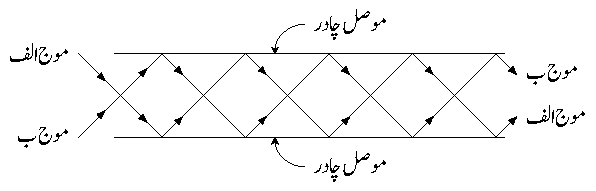
\includegraphics{figWaveguidesTwoConductingSheetsTwoTEMwaves}
\caption{شعاعیں دو چادروں کے درمیان بار بار انعکاس کرتی حرکت کرتی ہیں۔}
\label{شکل_مویج_شعاع_انعکاس_کرتی_حرکت_کرتی_ہے}
\end{figure}
%
\begin{figure}
\centering
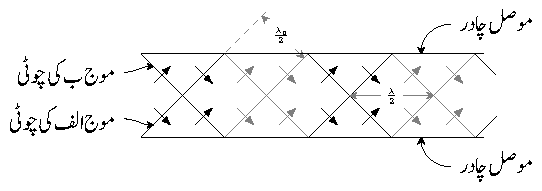
\includegraphics{figWaveguidesTwoConductingSheetsTwoTEMwavesWavefronts}
\caption{موجوں کی چوٹیاں، نشیب، خالی خلاء اور مویج میں طول موج۔}
\label{شکل_مویج_خالی_خلاء_اور_میوج_طول-موج}
\end{figure}

اگرچہ ہم دو عدد عرضی برقی و مقناطیسی \تحریر{TEM} امواج کی بات کرتے آ رہے ہیں، درحقیقت ان کا مجموعہ بلند درجی \تحریر{TE} انداز کی موج ہے۔بلند درجی انداز کے موج کی اہم خصوصیت  یہ ہے کہ اس کا طول موج ایک مخصوص حد سے کم ہونا لازم ہے۔ایسا نہ ہونے کی صورت میں یہ مویج سے نہیں گزر سکتی۔طول کی یہ حد \اصطلاح{انقطاعی طول}\فرہنگ{انقطاعی طول}\فرہنگ{طول!انقطاعی}\حاشیہب{cutoff wavelength}\فرہنگ{cutoff wavelength}\فرہنگ{wavelength!cutoff} پکاری جاتی ہے۔ آئیں انقطاعی طول حاصل کریں۔

 \begin{figure}
\centering
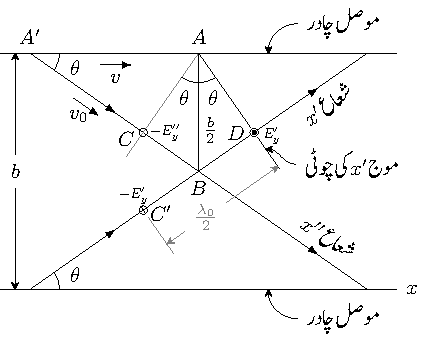
\includegraphics{figWaveguidesTwoConductingSheetsCutoffWavelength}
\caption{متوازی لامحدود وسعت کے چادروں کے مویج میں میدان کے اجزاء۔}
\label{شکل_مویج_متوازی_چادر_مویج_اجزاء_میدان}
\end{figure}

شکل \حوالہ{شکل_مویج_متوازی_چادر_مویج_اجزاء_میدان} میں \تحریر{TE} موج کے دو \تحریر{TEM} اجزاء دکھائے گئے ہیں جو \عددیء{x'} اور \عددیء{x''} سمت میں گامزن ہیں۔دونوں جزو موصل چادر یعنی \عددیء{x} محدد کے ساتھ \عددیء{\theta} زاویہ بناتے ہیں۔برقی میدان صفحہ کے عمودی \عددیء{y} محدد کی سمت میں ہے۔چادروں کے درمیان فاصلہ \عددیء{b} ہے۔نقطہ \عددیء{D} پر موج \عددیء{x'} کی چوٹی ہے لہٰذا یہاں برقی میدان \عددیء{E_y'} مثبت  قیمت رکھتا ہے جو صفحہ کے عمودی باہر کو ہے اور جسے گول دائرے میں بند نقطے سے ظاہر کیا گیا ہے۔ اس نقطے پر لکیر \عددیء{AD} لہر کی چوٹی ظاہر کرتی ہے۔عین اسی لمحہ نقطہ \عددیء{C} پر موج \عددیء{x''} کا نشیب ہے جسے گول دائرے میں بند صلیبی نشان سے ظاہر کیا گیا ہے۔اس لہر کے نشیب کو ہلکی سیاہی میں لکیر \عددیء{AC} سے ظاہر کیا گیا ہے۔ایک لہر کی چوٹی اور دوسرے لہر کا نشیب نقطہ \عددیء{A} پر مل کر صفر میدان پیدا کرتے ہیں۔ہم جانتے ہیں کہ عین دو چادروں کے درمیان دونوں امواج کی چوٹیاں مل کر دگنا میدان پیدا کرتی ہیں۔اس نقطے کو شکل میں \عددیء{B} سے ظاہر کیا گیا ہے۔یوں موج \عددیء{x''} کا نشیب \عددیء{C} پر جبکہ اس کی چوٹی \عددیء{B} پر ہے۔اس طرح ان نقطوں کے درمیان فاصلہ طول موج کا چوتھا حصہ ہو گا۔اسی طرح \عددیء{BD} اور \عددیء{C'B} بھی طول موج کے چوتھائی برابر  ہیں
\begin{align}
BC=BC'=BD=\frac{\lambda_0}{4}
\end{align}
جہاں لامحدود خلاء میں \تحریر{TEM} موج کا طول موج \عددیء{\lambda_0} ہے اور یہ خلاء اسی مادے سے بھری ہے جو دو چادروں کے درمیان پایا جاتا ہے۔موصل چادر پر ایک موج کی کوئی بھی چوٹی اور دوسری موج کا کوئی بھی نشیب مل کر صفر میدان پیدا کر سکتے ہیں۔یوں مندرجہ بالا مساوات کی عمومی شکل
\begin{align}\label{مساوات_مویج_چوٹی_نشیب_ختم_عمومی}
BC=\frac{n \lambda_0}{4}
\end{align}
ہے جہاں \عددیء{n=1,2,3,\cdots} ہو سکتے ہیں۔جفت \عددیء{n} کی صورت میں دو چادروں کے عین درمیان برقی میدان صفر حاصل ہو گا جبکہ طاق \عددیء{n} کی صورت میں یہاں میدان دگنا ہو گا۔ان حقائق ہر تفصیلاً جلد بات کی جائے گی۔شکل \حوالہ{شکل_مویج_متوازی_چادر_مویج_اجزاء_میدان} میں تکون \عددیء{ABC} سے
\begin{align*}
AB \sin \theta = \frac{b}{2}\sin \theta =\frac{n \lambda_0}{4}
\end{align*}
یعنی
\begin{align}\label{مساوات_مویج_طول_اور_درجہ_انداز}
\lambda_0 = \frac{2b}{n} \sin \theta
\end{align}
لکھا جا سکتا ہے جہاں لمبائی \عددیء{BC} کے لئے مساوات \حوالہ{مساوات_مویج_چوٹی_نشیب_ختم_عمومی} استعمال کیا گیا۔اس مساوات کے تحت زیادہ سے زیادہ طول موج \عددیء{\lambda_{0c}} کی قیمت \عددیء{\sin \theta=1} یعنی \عددیء{\theta=90^{\circ}} پر
\begin{align}\label{مساوات_مویج_طول_موج_بالمقابل_درجہ_موج}
\lambda_{0c}=\frac{2b}{n}
\end{align}
 حاصل ہوتی ہے جس سے \عددیء{n} کی ہر قیمت کے مقابل طول کی انقطاعی قیمت حاصل کی جا سکتی ہے۔جب \عددیء{n=1} ہو تب
 \begin{align}
\lambda_{0c}=2b
\end{align}
حاصل ہوتا ہے۔یہ کم تر درجے کی \تحریر{TE} موج کا انقطاعی طول ہے جو ان چادروں کے درمیان صفر کر سکتی ہے۔یہ مساوات کہتا ہے کہ چادروں کے درمیان فاصلہ کم از کم آدھے طول کے برابر ہو گا تو موج چادروں کے درمیان سے گزر پائے گی۔

\عددیء{n=1} کو بلند درجی \تحریر{TE} امواج کا کم تر درجہ کہا جاتا ہے۔\عددیء{n=2} اس سے ایک قدم بلند  درجے کی موج کہلائے گی اور اس کا انقطاعی طول
\begin{align}
\lambda_{0c}=b
\end{align}
ہو گا۔یوں \عددیء{n=2} درجے کی \تحریر{TE} موج کے گزرنے کا لئے چادروں کے درمیان کم از کم فاصل موج کے طول کے برابر ضروری ہے۔اسی طرح \عددیء{n=3} کے لئے \عددیء{\lambda_{0c}=\tfrac{2b}{3}} حاصل ہوتا ہے، وغیرہ وغیرہ۔

مساوات \حوالہ{مساوات_مویج_طول_موج_بالمقابل_درجہ_موج} اور مساوات \حوالہ{مساوات_مویج_طول_اور_درجہ_انداز} کو ملا کر
\begin{align}
\lambda_0=\lambda_{0c} \sin \theta
\end{align}
یا
\begin{align}
\theta=\sin^{-1}\frac{\lambda_0}{\lambda_{0c}}
\end{align}
لکھا جا سکتا ہے۔یوں کسی بھی درجے کی موج کا انقطاعی زاویہ \عددیء{\theta=90^{\circ}} حاصل ہوتا ہے۔اس زاویے پر موج  دونوں چادروں کے مابین، \عددیء{x} تبدیل کئے بغیر،  انعکاس کرتی رہتی ہے۔یوں چادروں کے درمیان ساکن موج پیدا ہوتی ہے جو \عددیء{x} سمت میں طاقت منتقل نہیں کر سکتی۔اگر طول موج \عددیء{\lambda_0} انقطاعی طول موج \عددیء{\lambda_{0c}} سے قدر کم ہو تب \عددیء{\theta} کی قیمت \عددیء{90^{\circ}} سے کم ہو گی اور موج، بار بار انعکاس کرتی ہوئی، چادروں کے درمیان \عددیء{x} سمت میں حرکت کر پائے گی۔جیسے شکل \حوالہ{شکل_مویج_طول_موج_اور_زاویہ_انعاکس} میں دکھایا گیا ہے، طول موج مزید کم کرنے سے زاویہ مزید کم ہوتا ہے۔آخر کار انتہائی کم طول موج پر صورت حال لامحدود خلاء میں موج کے حرکت مانند ہو جاتی ہے اور یہ شعاع کی طرح چادروں کے درمیان سیدھا گزرنے کے قابل ہو جاتی ہے۔

\begin{figure}
\centering
\begin{subfigure}{0.4\textwidth}
\centering
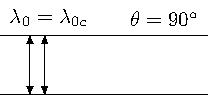
\includegraphics{figWaveguidesTwoConducorsAngleNinty}
\caption{طول موج، عین انقطاعی طول موج کے برابر ہے۔}
\end{subfigure}%
%
\begin{subfigure}{0.4\textwidth}
\centering
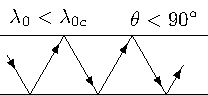
\includegraphics{figWaveguidesTwoConducorsAngleAbitLessThanNinty}
\caption{طول موج، انقطاعی طول موج سے قدر کم ہے۔}
\end{subfigure}%

\begin{subfigure}{0.4\textwidth}
\centering
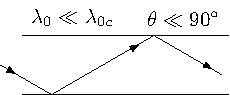
\includegraphics{figWaveguidesTwoConducorsAngleMuchLessThanNinty}
\caption{طول موج مزید کم کرنے سے زاویہ بھی مزید کم ہوتا ہے۔}
\end{subfigure}%
\begin{subfigure}{0.4\textwidth}
\centering
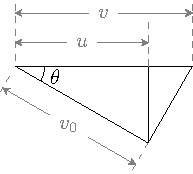
\includegraphics{figWaveguidesTwoConducorsPhaseGroupVelocities}
\caption{مختلف اقسام کے رفتار کا تعلق۔}
\end{subfigure}%
\caption{طول موج اور انعکاس موج کے زاویے۔ مختلف اقسام کے رفتاروں کا آپس میں تعلق۔}
\label{شکل_مویج_طول_موج_اور_زاویہ_انعاکس}
\end{figure}

شکل \حوالہ{شکل_مویج_متوازی_چادر_مویج_اجزاء_میدان} میں \تحریر{TEM} امواج کی \اصطلاح{دوری رفتار}\فرہنگ{دوری!رفتار}\فرہنگ{رفتار!دوری}\حاشیہب{phase velocity}\فرہنگ{phase velocity} \عددیء{v_0} لامحدود خلاء میں آزاد موج کی دوری رفتار
\begin{align}
v_0=\frac{1}{\sqrt{\mu \epsilon}} \quad (\si{\meter \per \second})
\end{align}
ہی ہے جہاں خلاء کا مقناطیسی مستقل \عددیء{\mu} اور اس کا برقی مستقل \عددیء{\epsilon} ہیں۔شکل \حوالہ{شکل_مویج_طول_موج_اور_زاویہ_انعاکس}-د میں \تحریر{TE} موج کی \عددیء{x} سمت میں دوری رفتار \عددیء{v} ہے۔\تحریر{TE} موج کی چوٹی یا نشیب یا کوئی اور زاویائی نقطہ اس رفتار سے \عددیء{x} سمت میں حرکت کرتا نظر آئے گا۔ان دو اقسام کے رفتار کا تعلق شکل \حوالہ{شکل_مویج_طول_موج_اور_زاویہ_انعاکس}-د سے
\begin{align}
\frac{v_0}{v}=\cos \theta
\end{align}
لکھا جا سکتا ہے جس سے
\begin{align}\label{مساوات_مویج_دوری_رفتار_تعلق_الف}
v=\frac{v_0}{\cos \theta}=\frac{1}{\sqrt{\mu \epsilon} \cos \theta} \quad \quad \si{\meter\per\second}
\end{align}
حاصل ہوتا ہے۔اس مساوات کے تحت جیسے جیسے طول موج کو انقطاعی طول موج کے قریب لایا جائے، ویسے ویسے \تحریر{TE} موج کی دوری رفتار کی قیمت بڑھتی ہے حتٰی کہ عین \عددیء{\lambda_{0c}} پر دوری رفتار لامحدود قیمت اختیار کر لیتی ہے۔اس کے برعکس جیسے جیسے طول موج کو کم کیا جائے، یعنی جیسے جیسے \عددیء{\theta} کو کم کیا جائے، ویسے ویسے \تحریر{TE} موج کی دوری رفتار \تحریر{TEM} کے دوری رفتار کے قریب ہو گی حتٰی کہ انتہائی کم طول موج یعنی انتہائی بلند تعدد کے موج کی صورت میں یہ قیمت \عددیء{v_0} کے برابر ہو جائے گی۔ یوں مویج میں بند، بلند درجی موج کا دوری رفتار \تحریر{TEM} موج کے دوری رفتار سے زیادہ یا اس کے برابر ممکن ہے۔طاقت کی منتقلی انعکاس کرتی موج کے \اصطلاح{مجموعی رفتار}\فرہنگ{مجموعی رفتار}\فرہنگ{رفتار!مجموعی}\حاشیہب{group velocity}\فرہنگ{group velocity} سے ہوتی ہے جسے شکل میں \عددیء{u} سے ظاہر کیا گیا ہے۔شکل \حوالہ{شکل_مویج_طول_موج_اور_زاویہ_انعاکس}-د سے
\begin{align}\label{مساوات_مویج_دوری_رفتار_تعلق_ب}
u=v_0 \cos \theta
\end{align}
لکھا جا سکتا ہے لہٰذا طاقت کی منتقلی کی رفتار \تحریر{TEM} کے رفتار سے کم یا اس کے برابر ممکن ہے۔طاقت کسی صورت بھی \تحریر{TEM} موج کی رفتار سے زیادہ رفتار پر منتقل کرنا ممکن نہیں ہے۔یہ حقیقت آئن سٹائن کے قانون کے عین مطابق ہے جس کے تحت کوئی بھی چیز رفتار شعاع سے تجاوز نہیں کر سکتی۔یاد رہے کہ \تحریر{TE} موج کی دوری رفتار درحقیقت کسی چیز کی منتقلی نہیں کرتی لہٰذا اس کی قیمت \عددیء{v_0} سے بڑھ سکتی ہے۔مساوات \حوالہ{مساوات_مویج_دوری_رفتار_تعلق_الف} اور مساوات \حوالہ{مساوات_مویج_دوری_رفتار_تعلق_ب}  کو ملا کر 
\begin{align}\label{مساوات_مویج_دوری_رفتار_تعلق_پ}
u v =v_0^2
\end{align}
حاصل ہوتا ہے۔

دو چادروں میں بند ہونے سے \تحریر{TEM} موج کا تعدد تبدیل نہیں ہوتا۔اسی طرح ایسے دو یکساں تعدد کے امواج سے حاصل \تحریر{TE} موج کا تعدد بھی وہی رہتا ہے۔چونکہ طول موج ضرب تعدد کا حاصل رفتار کے برابر ہوتا ہے لہٰذا مساوات \حوالہ{مساوات_مویج_دوری_رفتار_تعلق_الف} کو
\begin{align*}
f \lambda=\frac{f \lambda_0}{\cos \theta}
\end{align*}
لکھا جا سکتا ہے جس سے
\begin{align*}
\lambda=\frac{\lambda_0}{\cos \theta}
\end{align*}
حاصل ہوتا ہے جو بلند درجہ موج کے طول \عددیء{\lambda} اور آزاد موج کے طول \عددیء{\lambda_0} کا تعلق ہے۔

\begin{figure}
\centering
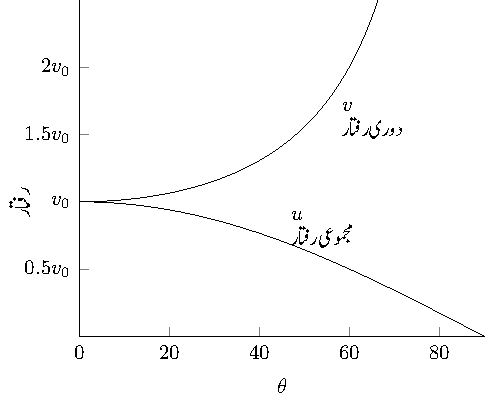
\includegraphics{figWaveguidesTwoConducorsPhaseGroupVelocitiesGraphicalView}
\caption{دوری اور مجموعی رفتار بالمقابل زاویہ موج۔}
\label{شکل_مویج_دوری_مجموعی_رفتار_بالمقابل_زاویہ}
\end{figure} 

شکل \حوالہ{شکل_مویج_دوری_مجموعی_رفتار_بالمقابل_زاویہ} میں دوری رفتار بالمقابل زاویہ موج اور مجموعی رفتار بالمقابل زاویہ موج دکھائے گئے ہیں۔جیسے جیسے \عددیء{\theta} کی قیمت \عددیء{90^{\circ}} کے قریب آتی ہے ویسے ویسے دوری رفتار کی قیمت لامحدود جبکہ مجموعی رفتار کی قیمت صفر کے قریب تر ہوتی ہے۔

حقیقت میں دو متوازی لامحدود وسعت کے چادروں پر مبنی مویج کہیں نہیں پایا جاتا۔حقیقی مویج عموماً کھوکھلے مستطیل یا کھوکھلے نالی کے اشکال رکھتے ہیں۔
